\documentclass[]{interact}

\usepackage[outdir=./]{epstopdf}% To incorporate .eps illustrations using PDFLaTeX, etc.
\usepackage[caption=false]{subfig}% Support for small, `sub' figures and tables
%\usepackage[nolists,tablesfirst]{endfloat}% To `separate' figures and tables from text if required
%\usepackage[doublespacing]{setspace}% To produce a `double spaced' document if required
%\setlength\parindent{24pt}% To increase paragraph indentation when line spacing is doubled

%\usepackage[longnamesfirst,sort]{natbib}% Citation support using natbib.sty
%\bibpunct[, ]{(}{)}{;}{a}{,}{,}% Citation support using natbib.sty
%\renewcommand\bibfont{\fontsize{10}{12}\selectfont}% To set the list of references in 10 point font using natbib.sty

\usepackage[natbibapa,nodoi]{apacite}% Citation support using apacite.sty. Commands using natbib.sty MUST be deactivated first!
%\setlength\bibhang{12pt}% To set the indentation in the list of references using apacite.sty. Commands using natbib.sty MUST be deactivated first!
%\renewcommand\bibliographytypesize{\fontsize{10}{12}\selectfont}% To set the list of references in 10 point font using apacite.sty. Commands using natbib.sty MUST be deactivated first!

%\theoremstyle{plain}% Theorem-like structures provided by amsthm.sty
%\newtheorem{theorem}{Theorem}[section]
%\newtheorem{lemma}[theorem]{Lemma}
%\newtheorem{corollary}[theorem]{Corollary}
%\newtheorem{proposition}[theorem]{Proposition}

%\theoremstyle{definition}
%\newtheorem{definition}[theorem]{Definition}
%\newtheorem{example}[theorem]{Example}

%\theoremstyle{remark}
%\newtheorem{remark}{Remark}
%\newtheorem{notation}{Notation}


%\documentclass{amsart}[12pt]
%\usepackage{amsmath, amsfonts, natbib, array, textcomp, graphicx}
%\oddsidemargin=0in \evensidemargin=0in
%\textwidth=6.6in \textheight=8.7in
\usepackage{mathtools, fix-cm}%lmodern,
% \usepackage{csvsimple}
\title{A variation on the Chamberlin Trimetric map projection}
%\author{B R S Recht}
\author{Author}
\date{November 2020}

\begin{document}

\begin{abstract}
   A variation of the Chamberlin Trimetric map projection is presented,
   termed the Matrix Trimetric projection. The Matrix Trimetric projection
   amounts to a linear transformation of the squares of the distances
   from a given point to three control points. It is significantly more
   efficient to calculate than the Chamberlin projection, and allows for an
   inverse projection in the spherical approximation which requires numerical
   iteration of only one parameter. Comparisons between the two projections
   are made using a representative list of control points. The Chamberlin
   projection outperforms the Matrix projection on measures of angle deformation
   and scale deformation, but the reverse is true for a measure of distance
   deformation. In general the difference between the projections is small.

\end{abstract}
\maketitle

\section{Introduction}
A map projection is a projection from a sphere or an ellipsoid -- such as one
being used to model the surface of the Earth -- to the plane. Map projections
that preserve angles are called conformal; ones that preserve the relative area
of shapes may be termed authalic, equal-area, equiareal or equivalent. No map
projection preserves distances between all points, but a map projection that
preserves distances along certain geodesics may be termed equidistant. All map
projections introduce some form of distortion: no map projection may be both
conformal and authalic.\citep{snyder87}
A compromise map projection is one that is neither conformal, authalic,
or equidistant, but seeks to balance different kinds of distortion.

The Chamberlin Trimetric projection is a compromise map projection that achieves
a balance between distortions in area, angle, and distance. It is named for
Wellman Chamberlin, a chief cartographer for the National Geographic
Society, which has published wall and atlas maps using this projection. The
Chamberlin projection is appropriate for mapping whole continents and large
portions of continents. The Chamberlin projection has a simple geometric
construction, shown in Figure \ref{fig:chamberlin}. Three control points on the
globe are specified, and a triangle in the plane is constructed having the same
distances between its vertices as the true distances between the points on the
globe. True distances from those control points to a given point on the globe
are measured, and arcs are drawn at those distances from their respective points
in the plane. The arcs form a small triangle: a point in that triangle is chosen
as the projection of the original point.\citep{christensen} Originally, in the
1950s when manual plotters were used, the exact definition of this point was not
important, but \citet{christensen} and most modern implementations
(e.g. \citet{proj}) use the centroid of the small triangle.
Thus, the Chamberlin projection is a form of triangulation:
it is also a cousin of the two-point equidistant projection.\citep{snyder89}

\begin{figure}%[!htbp]
  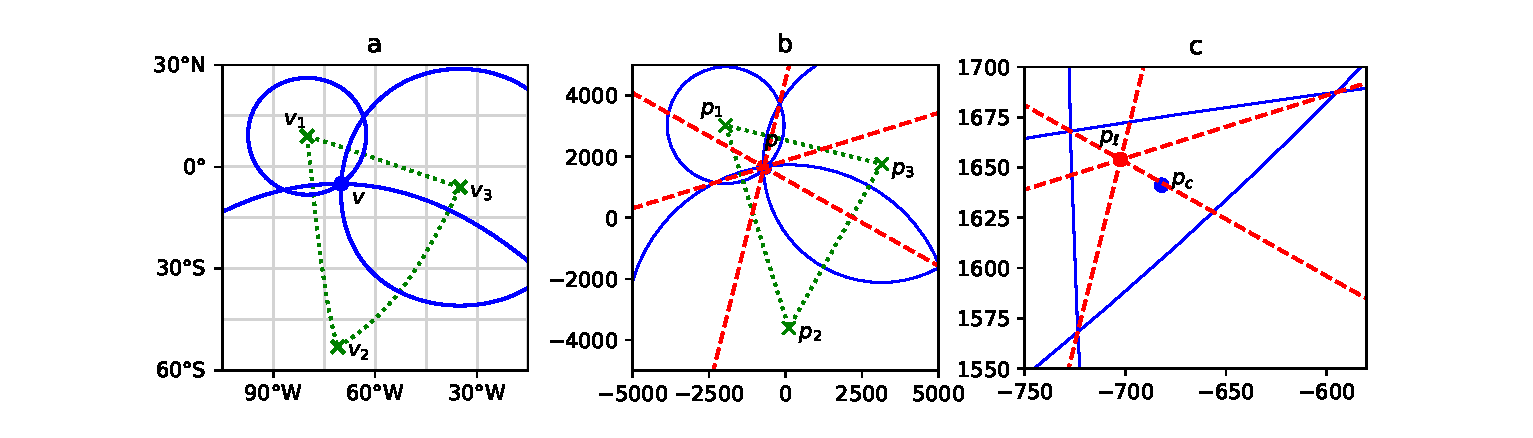
\includegraphics[width=\textwidth]{construction}
  \caption{Construction of the Chamberlin and Matrix Trimetric projections.
  Plot 1a is in equirectangular projection. Plot 1b is the projection
  to the plane. Plot 1c is the same as plot 1b, zoomed in to the small
  triangle created by the three circles. $\mathbf p_c$ is the point projected
  by the Chamberlin projection and $\mathbf p_m$ is the point projected
  by the Matrix Trimetric projection. Green solid lines indicate the control
  triangles, the circles are blue dots, and the perpendiculars are red dashes.}
  \label{fig:chamberlin}
\end{figure}

The geometric nature of this construction result in a somewhat involved
algorithmic form for the Chamberlin Trimetric projection. As commented on in
\citet{christensen}, the algorithmic form has special cases to handle when the
given point lies at a control point, or on an edge of the triangle with vertices
at the control points. This also makes analysis of the projection somewhat more
difficult, although numerical analysis of the distortion can be performed.

This text presents a new map projection called the Matrix Trimetric projection.
A geometric construction related to the Chamberlin Trimetric results in a map
projection that is very similar but has a simpler analytical formula. The
formula is simply the product of a matrix with a vector whose values are the
square of the distances from the given point to the control points, thus the
name. The differences between the Matrix Trimetric and Chamberlin projections
are difficult to notice with the naked eye. The Matrix Trimetric projection
introduces slightly more distortion in scale and angle, but less in a distance
measurement that will be defined later.

\section{Definitions and assumptions}
We use the spherical approximation to the Earth. For this text, we assume a
sphere with a radius of 6,371 km. The Chamberlin and Matrix projections are
compromise projections, and do not perfectly preserve angle, area, or distance.
For most practical ellipsoids, distortions due to the spherical approximation
are negligible compared to distortions due to the projection itself. If desired,
one can use an ellipsoid for distance calculations: the form of the forward
formula does not change, but the inverse formula is no longer valid. One can
also use an auxiliary latitude: see \citet{snyder87} for details.

$\mathbf v$ and subscripted versions shall denote points on the sphere, and
$\mathbf p = [x,~y]$ and subscripted versions shall denote points in the
Euclidean plane. Representing the points on the sphere as a unit vector allows
one to apply the tools of linear algebra. Refer to a basic text on linear
algebra, such as \citet{strang80}, if needed. Let latitude be $\varphi$ and
longitude be $\lambda$, then latitude and longitude can be converted to a unit
vector as so:
$$
\mathbf v =
\begin{bmatrix*}
  x \\y\\ z
\end{bmatrix*}
=
\begin{bmatrix*}
 \cos(\varphi) \cos(\lambda) \\
 \cos(\varphi) \sin(\lambda) \\
 \sin(\varphi)
\end{bmatrix*}.
$$
The conversion from a unit vector to latitude and longitude is:
\begin{equation}\begin{split}
  \varphi =& \arctan\left(z, \sqrt{y^2 + x^2}\right) \\
  \lambda =& \arctan\left(y, x\right)
\end{split}\end{equation}
where the 2-variable form of $\arctan$ is used, commonly called \texttt{arctan2}
or \texttt{atan2} in numeric libraries.

The spherical distance between two unit vectors is
$$
d\left(\mathbf v_i, \mathbf v_j\right) = R \arccos\left(\mathbf v_i \cdot \mathbf v_j\right)
=\arctan\left(\|\mathbf v_i \times \mathbf v_j\|, \mathbf v_i \cdot \mathbf v_j\right)
$$
where R is the radius of the Earth. The latter form, using the 2-variable form
of $\arctan$, is the most numerically stable. Euclidean distances are found
using the usual Euclidean norm: $\|\mathbf p_a - \mathbf p_b\|$.

Let $\mathbf v_1$, $\mathbf v_2$, $\mathbf v_3$ be control points on the sphere:
also let $\mathbf V$ be the matrix having $\mathbf v_i$ as its $i$th column. Let
$\mathbf p_1 = [x_1,~y_1]$ etc. be the control points on the plane. The
triangles with vertices at $\mathbf v_i$ or $\mathbf p_i$ are called the
control triangles (spherical or planar control triangle, respectively, if the
distinction is important). For this paper, the control triangle is not allowed
to have very small or zero area, e.g. the control points lie on a line or are
close together. We also exclude the case where all three points of the spherical
control triangle lie on the same great circle. None of these cases are typical
use cases for the Chamberlin projection. Note that the planar control triangle
is \textbf{not} the image of the spherical control triangle under either
projection. The image of the
spherical control triangle is slightly larger, and does not have straight edges.

$\mathbf p_i$ must be arranged such that
$d\left(\mathbf v_i, \mathbf v_j\right) = \|\mathbf p_i - \mathbf p_j\|$
for all $i$ and $j$ in $\{1, 2, 3\}$: the spherical length of the edges of the
spherical control triangle are equal to the Euclidean lengths of the planar
control triangles. Without loss of generality, also assume that
$\|\mathbf p_i\|$ is the same for all $i$, such that the center of the
circumcircle of the control triangle lies at the origin. This just removes a
translation in the plane in order to simplify the formulas; false northing and
easting can be added later. Given $\mathbf v_i$, $\mathbf p_i$ can be
constructed as follows. Let $i, j, k$ be a cyclic permutation of $\{1, 2, 3\}$,
and let $s_k = d\left(\mathbf v_i, \mathbf v_j\right)$. The circumradius of the Euclidean
triangle with sides of length $s_k$ is
\begin{equation}\label{eq:circumradius}
  C = \frac{\prod_i s_i}{\sqrt{\sum_i s_i^2 s_{i+1}^2 - s_i^4}}.
\end{equation}
From the (Euclidean) law of cosines,
the interior angle $\phi_i$ at each vertex is
\begin{equation}\label{eq:phi}
  \phi_i = \arccos \left( \frac{s_k^2 + s_j^2 - s_i^2}{2 s_k s_j}\right).
\end{equation}
Let $\mathbf P$ be the matrix whose $i$th column is the vector $\mathbf p_i$. Then a
set of points satisfying the requirements are given as so:
\begin{equation}\label{eq:planarctrlpts}
  \mathbf P = \begin{bmatrix*}[r]
  C \cos \left(2 \phi_1 \right) &
  C \cos \left(2 \phi_0 \right) &
  C \\
  C \sin \left(2 \phi_1 \right) &
  -C \sin \left(2 \phi_0 \right) &
  0 \\
\end{bmatrix*}.
\end{equation}
These points can be rotated about the origin as desired.

To measure distortion of area and angle, we use the area scale factor $s$ and
maximum angular deformation $\omega$ as defined in equations 12--15, 27, and 28
in section 4 of \citet{snyder87}. Derivatives are estimated numerically using
second-order central differences on a 1-degree grid via the \texttt{gradient}
function in Numpy.\citep{numpy}
There is no standard measurement of distance distortion for map projections, as
most map projections fix one or no points. For the projections in this text,
it makes sense to measure distances from the control points. Let $r_i$ be the
distance from $\mathbf v_i$ to $\mathbf v$ on the sphere, as earlier, and let
$\ell_i$ be the distance from $\mathbf p_i$ to $\mathbf p$ in the plane.
The measure, denoted $D$, is the sum of differences in the distances
measured on projected and unprojected distances:
\begin{equation}
 D = \sum_i \left| r_i - \ell_i \right|.
\end{equation}

\section{Forward projection}

Let $r_i = d\left(\mathbf v_i, \mathbf v\right)$ be the spherical distance from
$\mathbf v_i$ to $\mathbf v$, but also the radius of a circle on the sphere
surface such that $\mathbf v_i$ is the center and $\mathbf v$ lies on the
circle's boundary. The Chamberlin projection draws a circle of radius $r_i$
around each point $\mathbf p_i$, forming a small triangle with circular arcs for
edges, and chooses a point $\mathbf p_c$ as the centroid of that small triangle.
Of course, each pair of circles intersects in at most two places, so the
implementation must take care to choose the point of intersection that
lies on the small triangle and not the other.

One can make two observations on this configuration of circles in the plane. One
is that the two points of intersection of each pair of circles are symmetric
about the triangle edge between the two control points. The other is that, if
one draws a line through the two points of intersection of each pair of circles,
that line is perpendicular to the triangle edge. These are the dashed red lines
in Figure \ref{fig:chamberlin}. Once the lines are drawn for each pair of
circles, the three lines appear to meet at the same point.
This can be proven with a simple triangle theorem sometimes attributed to
Carnot.\citep{posamentier}\citep{wohlgemuth} Although that point is not
necessarily within the small triangle, it is for most points within the control
triangle.

% Suppose that $\mathbf p_1 = [-1,0]$ and $\mathbf p_2 = [1,0]$. Then the points
% of intersection of the circles with radius $r_1$ and $r_2$ are given as so:
% \begin{equation}\begin{split}
% x =& \frac{r^2_1 - r^2_2}{4}\\
% y =& \pm \frac{1}{4} \sqrt{-
% \left(r_1 - r_2 - 2\right)
% \left(r_1 - r_2 + 2\right)
% \left(r_1 + r_2 - 2\right)
% \left(r_1 + r_2 + 2\right)}
% \end{split}\end{equation}
% Note that if the circles do not intersect, there is no real solution for $y$.
%
% If a line passing through the two points of intersection is drawn, it intersects
% the triangle edge from $\mathbf p_1$ to $\mathbf p_2$ perpendicularly at
% the point with $x$ as above and $y=0$: call that point $\mathbf p_{12}$. In
% general form, one can use linear interpolation to determine the point of
% perpendicular intersection $\mathbf p_{ij}$ as so:
% \begin{equation}\label{eq:pij}
% \mathbf p_{ij} = \mathbf p_i \frac{1-t_{ij}}{2} + \mathbf p_j \frac{1+t_{ij}}{2}
% \end{equation}
% \begin{equation}
% t_{ij} = \frac{r_i^2 - r_j^2}{\| \mathbf p_i - \mathbf p_j \|^2}
% \end{equation}
% Note that this is defined for all $r_i$ and $r_j$,
% regardless of whether the circles intersect.
%
% The lines passing through $\mathbf p_{ij}$ and parallel to the line from
% $p_i$ to $p_j$ all meet at the same point. This can be proven with a simple
% triangle theorem sometimes attributed to Carnot: such lines meet at a single
% point if and only if \citep{posamentier}\citep{wohlgemuth}
% \begin{equation}
%   \|\mathbf p_1 - \mathbf p_{12}\| +
%   \|\mathbf p_2 - \mathbf p_{23}\| +
%   \|\mathbf p_3 - \mathbf p_{31}\| =
%   \|\mathbf p_2 - \mathbf p_{12}\| +
%   \|\mathbf p_3 - \mathbf p_{23}\| +
%   \|\mathbf p_1 - \mathbf p_{31}\|
% \end{equation}
% for points $\mathbf p_{ij}$ lying on the edge between $\mathbf p_i$ and
% $\mathbf p_j$. Plugging in Equation \ref{eq:pij} and simplifying proves that
% these lines satisfy this theorem.
%
% The equation of the line passing from $\mathbf p_i$ to $\mathbf p_j$ is:
% \begin{equation}
% y (x_i - x_j) - x (y_i - y_j) - x_i y_j - x_j y_i = 0.
% \end{equation}
% Thus, the equation of the line perpendicular to that line and passing through
% the point $\mathbf p_{ij}$ can be found to be
% \begin{equation}
% y (y_i - y_j) + x (x_i - x_j) + \frac{r_i^2 - r_j^2}{2} = 0.
% \end{equation}

The equations of each perpendicular line, taken together, create a linear
system. It is an overdetermined system of 3 equations in 2 variables, but since
all 3 lines meet at the same point, it has a solution. Ultimately this system
can be solved for $\mathbf p_m$ to define a forward map projection as follows.
\begin{equation}\label{eq:forward}
\mathbf p_m = \mathbf M \begin{bmatrix*} r^2_1 & r^2_2 & r^2_3 \end{bmatrix*}^\top,
\end{equation}
\begin{equation}\label{eq:forwardm}
\mathbf M = \frac{1}{2T}
\begin{bmatrix*} y_3 - y_2 & y_1 - y_3 & y_2 - y_1 \\
x_2 - x_3 & x_3 - x_1 & x_1 - x_2 \end{bmatrix*} = \frac{1}{2T}
\begin{bmatrix*}[r] 0 & -1  \\
1 & 0 \end{bmatrix*}
\mathbf P
\begin{bmatrix*}[r] 0 & -1 & 1 \\
1 & 0 & -1 \\
-1 & 1 & 0 \end{bmatrix*},
\end{equation}
\begin{equation}\label{eq:forwardt}
T = \begin{vmatrix*} x_1 & x_2 & x_3 \\
 y_1 & y_2 & y_3 \\
 1 & 1 & 1
\end{vmatrix*}.
\end{equation}
$T$ is equal to twice the area of the Euclidean control triangle.

The matrix $\mathbf M$ has a (right) nullspace spanned by the vector
$[1, 1, 1]$. This implies the Matrix Trimetric projection is not one-to-one for
all possible values of $r_i$: for example, for any values of $r_i$ such that
$r_1 = r_2 = r_3$, then $\mathbf p_m = [0, 0]$. Both the Chamberlin and Matrix
Trimetric projections project the entire sphere to a bounded portion of the
plane. This can be termed the boundary of the projection. There is a region of
overlap that is mapped into the same area but in reverse orientation. That
region includes the antipodes of the control points.
In real applications, the overlap region can be excluded.

\section{Inverse projection}
Given $\mathbf p_m$, start to invert the projection as so:
\begin{equation}\label{eq:inverse}
\begin{bmatrix*} k_1 & k_2 & k_3

\end{bmatrix*}^\top = \mathbf M^+ \mathbf p_m,
\end{equation}
\begin{equation}\label{eq:inversem}
\mathbf M^+ = \frac{2}{3}
\begin{bmatrix*}[r] 2x_1 - x_2 - x_3 & 2y_1 - y_2 - y_3 \\
-x_1 + 2x_2 - x_3 & -y_1 + 2y_2 - y_3 \\
-x_1 - x_2 + 2x_3 & -y_1 - y_2 + 2y_3
\end{bmatrix*} = \frac{2}{3}
\begin{bmatrix*}[r] -2 & 1 & 1 \\
1 & -2 & 1 \\
1 & 1 & -2
\end{bmatrix*}
\mathbf P^\top
\end{equation}
$k_i = r^2_i - h$ for some value $h$. This is a general solution to inverting
Equation \ref{eq:forward}, thus the free parameter $h$. $\mathbf M^+$ is the
pseudoinverse of $\mathbf M$ and vice versa. Because $\mathbf M^+$ has a left
nullspace spanned by the vector $[1, 1, 1]$, it follows that $\sum_i k_i = 0$,
which can be used to skip some steps in calculating of $k_i$.

Plugging Equation \ref{eq:forward} into Equation \ref{eq:inverse} reveals that
$h = \frac{1}{3}\sum_i r^2_i$. Unfortunately, if one attempts to solve for
$r_i$ given $k_i$, they find another general solution with one free parameter,
putting them right back where they started. It turns out that information about
the sphere needs to be introduced to determine $r_i$ and $\mathbf v$.
%In the following, this is done using the spherical approximation,
%and the case of an ellipsoid is discussed.

%\subsection{With spherical approximation}

For the following, let $r_i$ have units of radians of arc on the surface of the
sphere, i.e. $R=1$. This does not affect the result or require unit conversion
in implementation, it just makes the derivation simpler. The circle of points
$\mathbf v$ at distance $r_0$ from a point $\mathbf v_0$ is simply the circle
where a plane intersects the sphere. This plane may be specified as
$\mathbf v_0 \cdot \mathbf v = \cos\left(r_0\right).$
Replacing $\mathbf v_0$ with $\mathbf v_i$ and $r_0$ with $r_i$ for each $i$
gives a linear system. Thus,
\begin{equation}\label{eq:inversev}
  \mathbf v = \mathbf V^{-1} \begin{bmatrix*} \cos\left(r_1\right) \\
  \cos\left(r_2\right) \\
  \cos\left(r_3\right)
  \end{bmatrix*}.
\end{equation}

For the point to lie on the unit sphere, $\|\mathbf v\| = 1$. Let $\mathbf c$
be a vector with $i$th component $\cos\left(r_i \right)$. Then,
$\mathbf c^\top \left(\mathbf V^\top \mathbf V\right )^{-1} \mathbf c = 1$.
Make the substitution
\begin{equation}\label{eq:inverser}
  r_i = \sqrt{k_i + h}.
\end{equation} We now have an equation with one unknown, $h$.

Some obvious bounds can be placed on $h$. In units of radians,
$0 \le r_i \le \pi$. Since this must hold for every $r_i$, it follows that
\begin{equation}
   -\min_i k_i \le h \le \pi^2 - \max_i k_i.
\end{equation}
Within these bounds, there may be at most two solutions for $h$. The solution
with smaller $h$ is the desired one, and the one with larger $h$ corresponds to
the overlap region.

Let
\begin{equation}\label{eq:inversefh}
f(h) = \mathbf c^\top \mathbf A \mathbf c - 1.
\end{equation}
where $\mathbf A = \left(\mathbf V^\top \mathbf V\right )^{-1}$
 is symmetric and positive semi-definite.
%See Figure \ref{fig:fh} for a plot of $f(h)$ for various points.
The derivative of $f(h)$ is
\begin{equation}\label{eq:inversefph}
  f'(h) = -\mathbf c^\top \mathbf A \mathbf b
\end{equation}
where $\mathbf b$ is a vector with $i$th component
$\mathrm{sinc}\left(\sqrt{k_i + h}\right)$.
Note that $f'(h)$ and $f(h)$ share many of the same terms, a fact that can be
exploited to make the calculation more efficient.

% the function $\mathrm{sinc} (x)$
% is defined as so:
% \begin{equation}
% \mathrm{sinc} (x) = \begin{cases}
%       1 & \text{if}\ x=0, \\
%       \frac{\sin x}{x} & \text{otherwise}.
%     \end{cases}
% \end{equation}

%If needed for numerical purposes, the compositions
%of trigonometric functions with square root can be smoothly extended to negative values:
%when $x<0$, $\cos \sqrt{x} = \cosh \sqrt{-x}$
%and $\mathrm{sinc}(\sqrt{x}) = \frac{\sin \sqrt{x}}{\sqrt{x}} = \frac{\sinh \sqrt{-x}}{\sqrt{-x}}$.

%\begin{figure}%[!htbp]
%  \includegraphics[width=\textwidth]{VariableH.png}
%  \caption{Plot of $f(h)$ for a number of points in the plane. Labels are
%  $x,y$ coordinates in thousands of kilometers.}
%  \label{fig:fh}
%\end{figure}
The lower solution for $\mathbf p_m = [0, 0]$ is a
global minimum for $h$, and can be calculated analytically as so:
\begin{equation}
  h_0 = \arccos \left(\frac{1}{\sqrt{\sum \mathbf A }} \right)^2
\end{equation}
where $\sum \mathbf A$ denotes the sum of all entries in the matrix $\mathbf A$.

Given all the preceding, Newton's method can be applied to solve for $h$.
A suitable initial condition is
\begin{equation}\label{eq:inverseh}
  h_{\min} = \max \left(h_0, -\min_i k_i \right),
\end{equation}
which appears to always result in convergence to the lower root of $f(h)$. One
could use $\frac{1}{3}\sum_i l^2_i$, where $l_i = |\mathbf p_m - \mathbf p_i|$
approximates $r_i$ fairly well, but for some $\mathbf p_m$ near the boundary
of the projection the iteration converges to the higher root.

A good approximation is achieved for points inside the control triangle within
only a few iterations. Convergence is somewhat slower further away from the
control triangle, and is worst at the boundary of the projection. This is
expected: at the boundary,
the lower solution and upper solution are the same and $f(h)=f'(h)=0$
so Newton's method converges at a merely linear rate.\citep{burden}

% \subsection{Without spherical approximation}
% The method for spheres is not extensible to ellipsoids. Geodesic
% circles cannot in general be described as the intersection of a plane and a
% surface. Also, we can no longer make the assumption that the Euclidean norm
% $\|\mathbf v\|$ is constant. In general, these sort of problems are harder on
% an ellipsoid than a sphere. Geodesic circles are usually calculated in most
% software by brute force: extending a number of lines a certain distance from a
% center point and using the endpoints as an approximation of the
% circle.\citep{FIXME} It is not surprising that an
% analytic form, or form with an easy numerical iteration, is not available here.
%
% The spherical approximation is reasonably close to an ellipsoidal
% calculation. Figure \ref{fig:roundtrip} demonstrates the results of performing
% the forward transformation with the ellipsoid and then transforming it back
% using the spherical inverse transformation, and then calculating the deviation
% in distance of each point. Within the control triangle, the
% deviation does not exceed 25 kilometers, and within the hemisphere containing the
% control triangle, no more than 60 near the south pole.
%
% \begin{figure}%[!htbp]
%   \includegraphics[width=\textwidth]{RoundTrip.png}
%   \caption{Deviation after round-trip transformation.
%   Units on contours are kilometers.}
%   \label{fig:roundtrip}
% \end{figure}

% \section{Derivation of Jacobians}
% The Jacobian of a projection is the matrix of derivatives
% \begin{equation}
%   \mathbf{J} =
%   \begin{bmatrix*}
%     \frac{\partial x}{\partial \lambda} &
%     \frac{\partial x}{\partial \phi} \\
%     \frac{\partial y}{\partial \lambda} &
%     \frac{\partial y}{\partial \phi}
%   \end{bmatrix*}
% \end{equation}
% Given the Jacobian $J$, the areal scale factor $s$ and maximum angular deformation
% $\omega$ can be calculated using equations 12-15, 27, and 28 in section 4 of
% \citep{snyder87}.
%
% Determining these derivatives requires some understanding of the differential
% geometry of the ellipsoid. Here we follow chapter 11 of \citep{strang12}.
% Let $e$ be the (first) eccentricity of the ellipsoid, then the second
% eccentricity $e'$ is defined as:
% \begin{equation}
%   e'^2 = \frac{e^2}{1-e^2}
%   %\qquad\qquad \mbox{(1.2)}
% \end{equation}
% There are two radii of curvature, the horizontal radius of curvature $M$ and
% the vertical radius of curvature $N$. On an oblate spheroid, $M \le N$.
% \begin{equation}
%   M = \frac{a\left(1-e^2\right)}{\left(1-e^2 \sin^2 \phi\right)^{\frac{3}{2}}}
%   %\qquad\qquad \mbox{(11.15)}
% \end{equation}
% \begin{equation}
%   N = \frac{a\sqrt{1-e'^2}}{\sqrt{1-e'^2 \cos^2 \phi}}
%   %\qquad \mbox{(unnumbered, between 1.16 and 1.17)}
% \end{equation}
% Finally, the differential equations for the line element $s$ are
% \begin{equation}
%   \frac{d \phi}{d s} = \frac{\cos \alpha}{M}
%   %\qquad\qquad \mbox{(1.63)}
% \end{equation}
% \begin{equation}
%   \frac{d \lambda}{d s} = \frac{\sin \alpha}{N \cos \phi}
%   %\qquad\qquad \mbox{(1.64)}
% \end{equation}
% and $\alpha$ is the azimuth at $\phi, \lambda$. These can obviously be inverted
% to give $\frac{d s}{d \phi}$ and $\frac{d s}{d \lambda}$.
%
% For the Matrix Trimetric projection, all we need to continue is the fact that
% $\frac{d s^2}{d \phi} = 2 s \frac{ds}{d \phi}$ (and similarly for $\lambda$).
%
%
%
% It can be shown that if and only if the scale factor $s$ is 0, then the determinant of the Jacobian above is 0.

\section{Comparison}
A software implementation of the Matrix Trimetric projection was implemented in
Python, using the libraries Numpy \citep{numpy}, Scipy \citep{scipy}, Pandas
\citep{pandas}, GeoPandas \citep{geopandas}, and their dependencies. The
implementation of the Chamberlin Trimetric projection comes from \citet{proj}.
Because the Chamberlin Trimetric and Matrix Trimetric projections are
implemented in different programming languages,
one compiled and one interpreted,
a comparison of computation time would be unfair and is not included here.

\citet{christensen} gave a list of control triangles for the Chamberlin
projection in that paper's Table 1. These serve as a set of test cases for
comparing the Chamberlin and Matrix projections. The control triangles are
repeated in this text's Table \ref{table:ctrlpts}. The length of each side and
the area of each triangle (with the spherical approximation given earlier)
is also given, and the control triangles are sorted by area.

\begin{table}
\begin{tabular}{ p{2.5cm} | p{1.5cm} p{1.5cm} p{1.5cm} | r r r | r }
Region & \multicolumn{3}{c}{Point} & \multicolumn{3}{c}{Side length} & Area \\
& 1 & 2 & 3 & 1 & 2 & 3 & \\
\hline
Canada \mbox{Atlas} & 98°13'W, 61°39'N & 135°W, 40°N & 55°W, 40°N & 6,560 & 3,761 & 3,449 & 5.28 \\
Canada Wall & 150°W, 60°N & 97°30'W, 50°N & 45°W, 60°N & 3,423 & 5,197 & 3,423 & 6.11 \\
NW South \mbox{America} & 69°W, 25°S & 55°W, 10°N & 85°W, 10°N & 3,284 & 4,261 & 4,177 & 6.70 \\
Australia & 134°E, 8°S & 110°E, 32°S & 158°E, 32°S & 4,487 & 3,643 & 3,643 & 6.76 \\
S South \mbox{America} & 43°W, 18°S & 72°W, 18°S & 72°W, 56°S & 4,225 & 4,874 & 3,064 & 6.77 \\
E South \mbox{America} & 63°33'W, 8°8'N & 58°33'W, 34°35'S & 35°13'W, 5°47'S & 4,000 & 3,502 & 4,779 & 7.25 \\
Europe Wall & 15°E, 72°N & 8°W, 33°N & 38°E, 33°N & 4,254 & 4,541 & 4,541 & 9.09 \\
South \mbox{America} Wall & 80°W, 9°N & 71°W, 53°S & 35°W, 6°S & 6,161 & 5,259 & 6,947 & 17.7 \\
North \mbox{America} Wall & 150°W, 55°N & 92°30'W, 10°N & 35°W, 55°N & 7,064 & 6,434 & 7,064 & 23.71 \\
Africa Wall & 19°3'W, 24°25'N & 20°E, 35°S & 59°3'E, 24°25'N & 7,783 & 7,785 & 7,783 & 32.38
\end{tabular}
\caption{Table of control triangles and their measurements. Side $n$ is opposite Point $n$.
Lengths are in km, and areas are in millions of square km.}
\label{table:ctrlpts}
\end{table}

For each control triangle, some summary statistics for $s$, $\omega$, and $D$
are calculated. These statistics are measured within the control triangles, and
should not be taken to summarize the entire map: for most of the triangles,
the region of interest extends outside the control triangle. Rather, the
statistics allow a quantitative comparison of the two projections. Some clear
trends appear in these figures, Figures \ref{fig:omegap}, \ref{fig:distancep},
and \ref{fig:scalep}. Note that the control triangles are sorted by
area in these figures as well, with low area at the bottom and high area at top.

\begin{figure}
  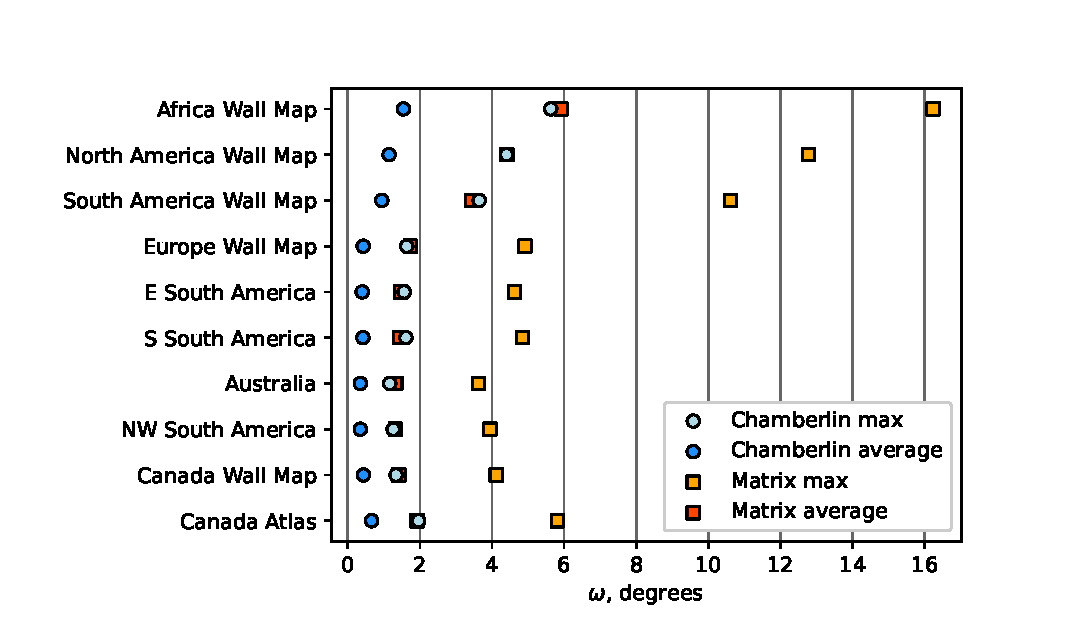
\includegraphics[width=\textwidth]{omegaplot}
  \caption{Comparison of angle distortion $\omega$.}
  \label{fig:omegap}
\end{figure}

As shown in Figure \ref{fig:omegap}, the Matrix projection consistently has a
larger $\omega$ than the Chamberlin projection: in fact, the maximum $\omega$
for Chamberlin is near the average $\omega$ for Matrix. Maximum and average
$\omega$ trend upwards with control triangle area, although asymmetry of the
control triangle has some influence too, as in the Canada triangles.
The maximum $\omega$ for Matrix is about 3 times that for Chamberlin, and
the average $\omega$ is about 3 to 4 times. However, for
moderately-sized triangles, the maximum $\omega$ values are small for both
projections, not exceeding 6°. Even for the large triangles -- Africa, North
America, and South America Wall Maps -- the maximum distortion is tolerable,
and the average does not exceed 6°.

\begin{figure}
  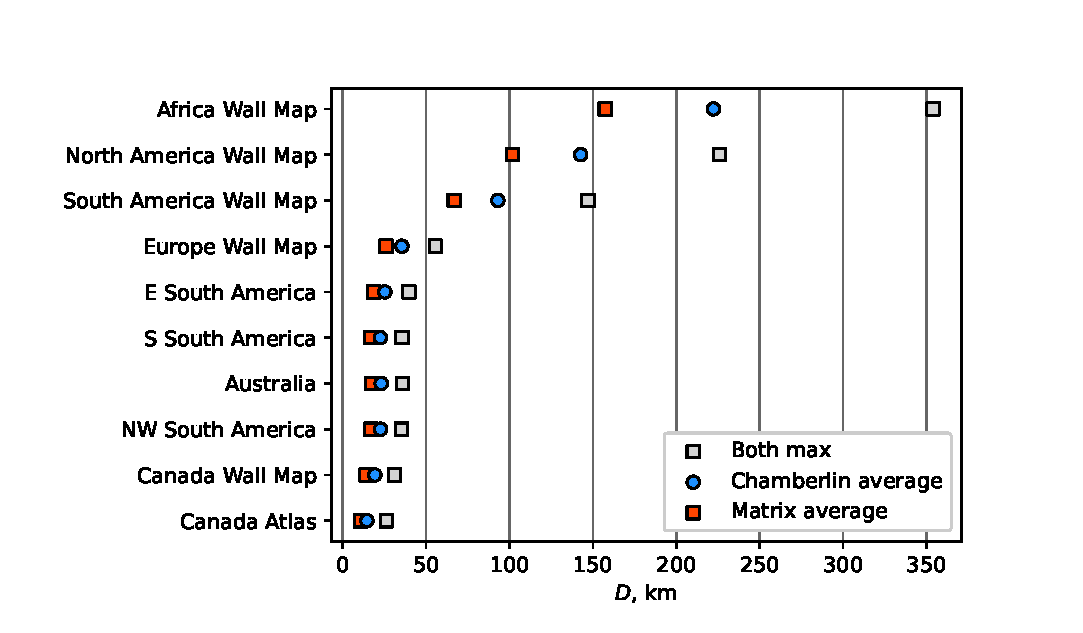
\includegraphics[width=\textwidth]{distanceplot}
  \caption{Comparison of total distance distortion $D$.}
  \label{fig:distancep}
\end{figure}

Distance distortion $D$ in Figure \ref{fig:distancep} shows an even clearer
trend, monotonically increasing with triangle area. Both projections have nearly
indistinguishable maximum $D$ values. The Matrix projection has consistently
lower average $D$ values than the Chamberlin: among these triangles, the maximum
$D$ for Chamberlin is about 1.35 to 1.4 times the maximum $D$ for Matrix. The
worst distortion,
Africa Wall Map's maximum $D$, is less than 5\% of its edge lengths, and
smaller control triangles have a maximum $D$ that is an even smaller percent.

\begin{figure}
  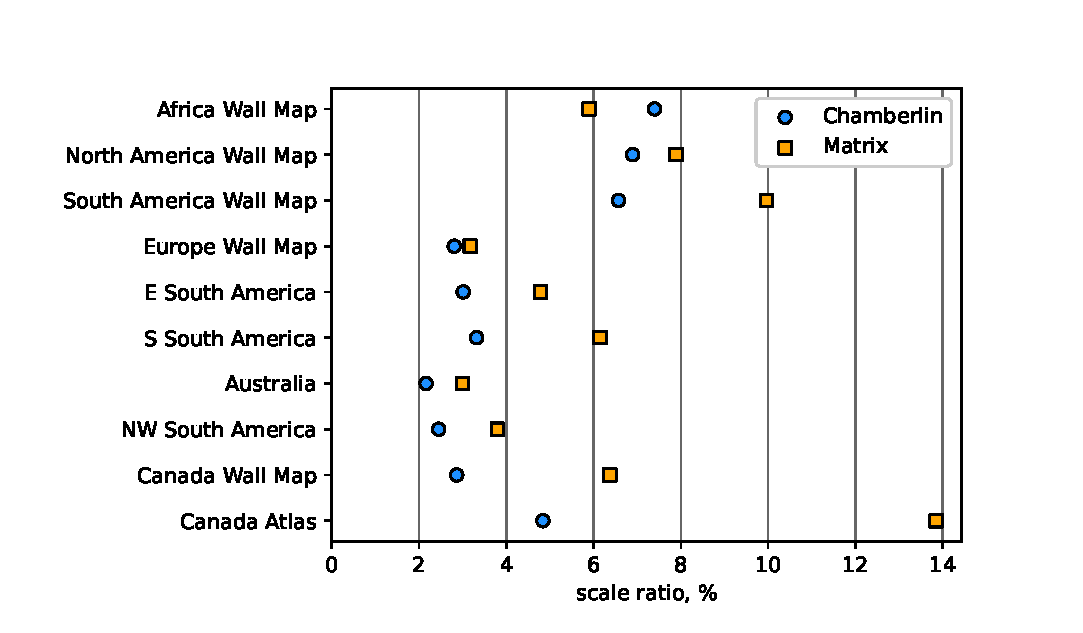
\includegraphics[width=\textwidth]{scaleplot}
  \caption{Comparison of area scale distortion $\frac{\max s}{\min s} - 1$.}
  \label{fig:scalep}
\end{figure}

As true 1:1 scale maps are rare, absolute values of $s$ are unimportant: the
quantity $\frac{\max s}{\min s} - 1$ is plotted in Figure \ref{fig:scalep}
instead. Scale distortion, $\frac{\max s}{\min s} - 1$, shows a less clear
trend. A combination of control triangle area and asymmetry influences this
value. In general, this value is higher for Matrix than for Chamberlin, but
not by any consistent factor, and for the large and symmetric Africa Wall Map
triangle the Matrix projection is lower than Chamberlin. The amount of scale
distortion is small for both: except for the very flat Canada Atlas triangle,
all values are below 10\%.

A comparison of the two projections using the South America Wall Map control
points is in Figure \ref{fig:proj}, using land mass shape files from
\citet{natearth}. The South America Wall Map control triangle is fairly
representative, being somewhat asymmetric but not too elongated or compressed.
The small part of Central America in the upper left is somewhat shifted between
the two maps, as is the western area near Ecuador and Peru, but no features on
either map are conspicuously distorted compared to the other. Figure
\ref{fig:tissot} shows ellipses of distortion spaced on a grid at steps of 15°
latitude and longitude. Distortion is somewhat more visible in this figure:
one can see that the Matrix projection introduces
slightly more shearing near the control points.

\begin{figure}%[!htbp]
  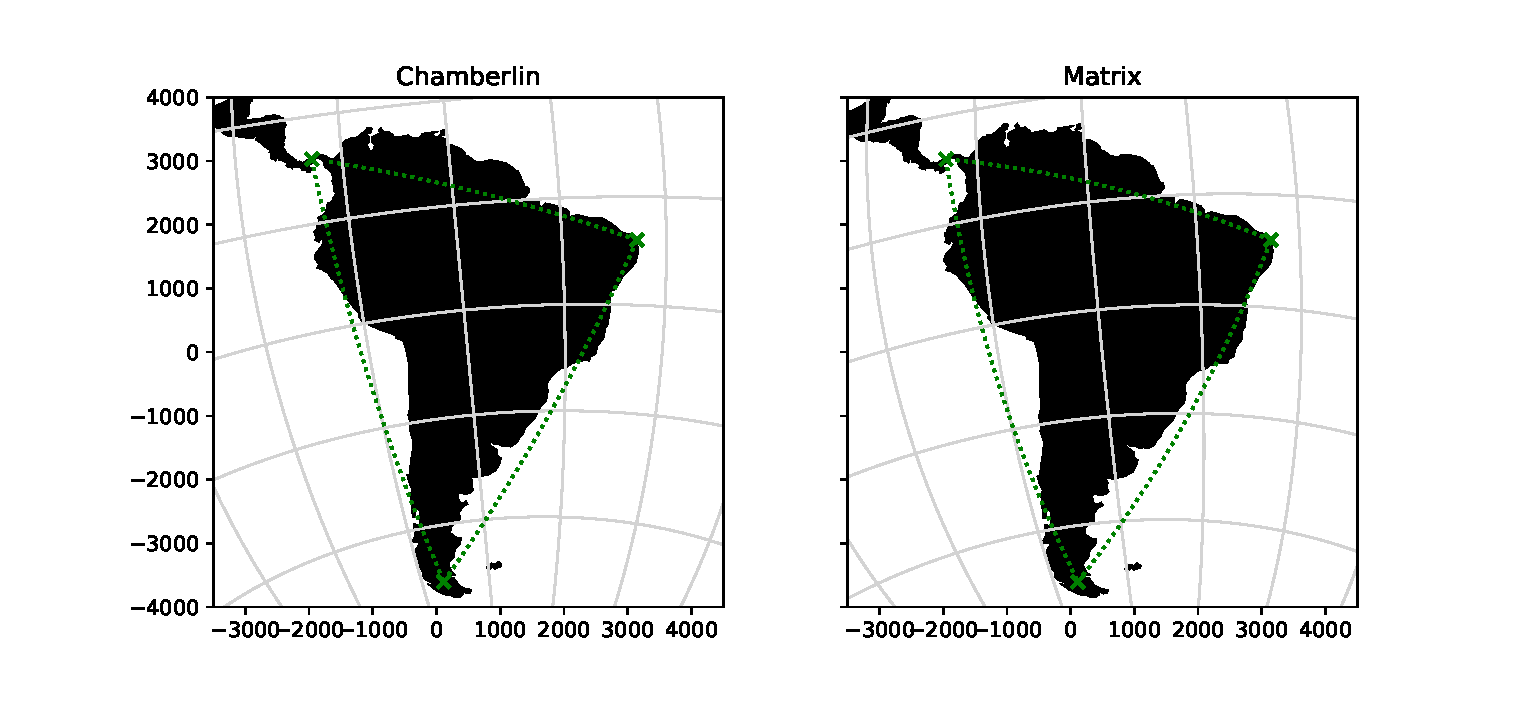
\includegraphics[width=\textwidth]{SA_Wall_Map_zoom}
  \caption{Projection of South America and surroundings.}
  \label{fig:proj}
\end{figure}

\begin{figure}%[!htbp]
  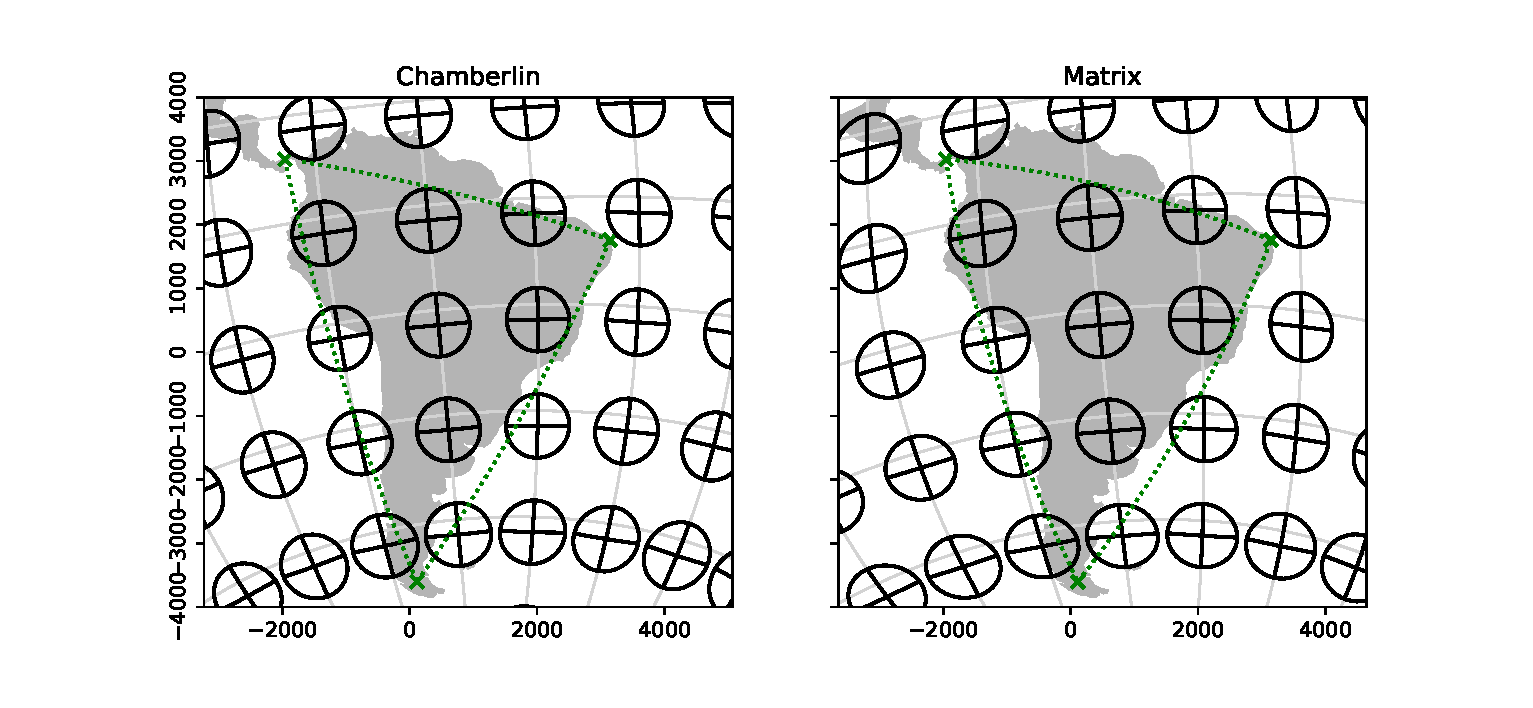
\includegraphics[width=\textwidth]{SA_Wall_Map_tissot}
  \caption{Ellipses of distortion, on a 15 degree grid.}
  \label{fig:tissot}
\end{figure}

\begin{figure}%[!htbp]
  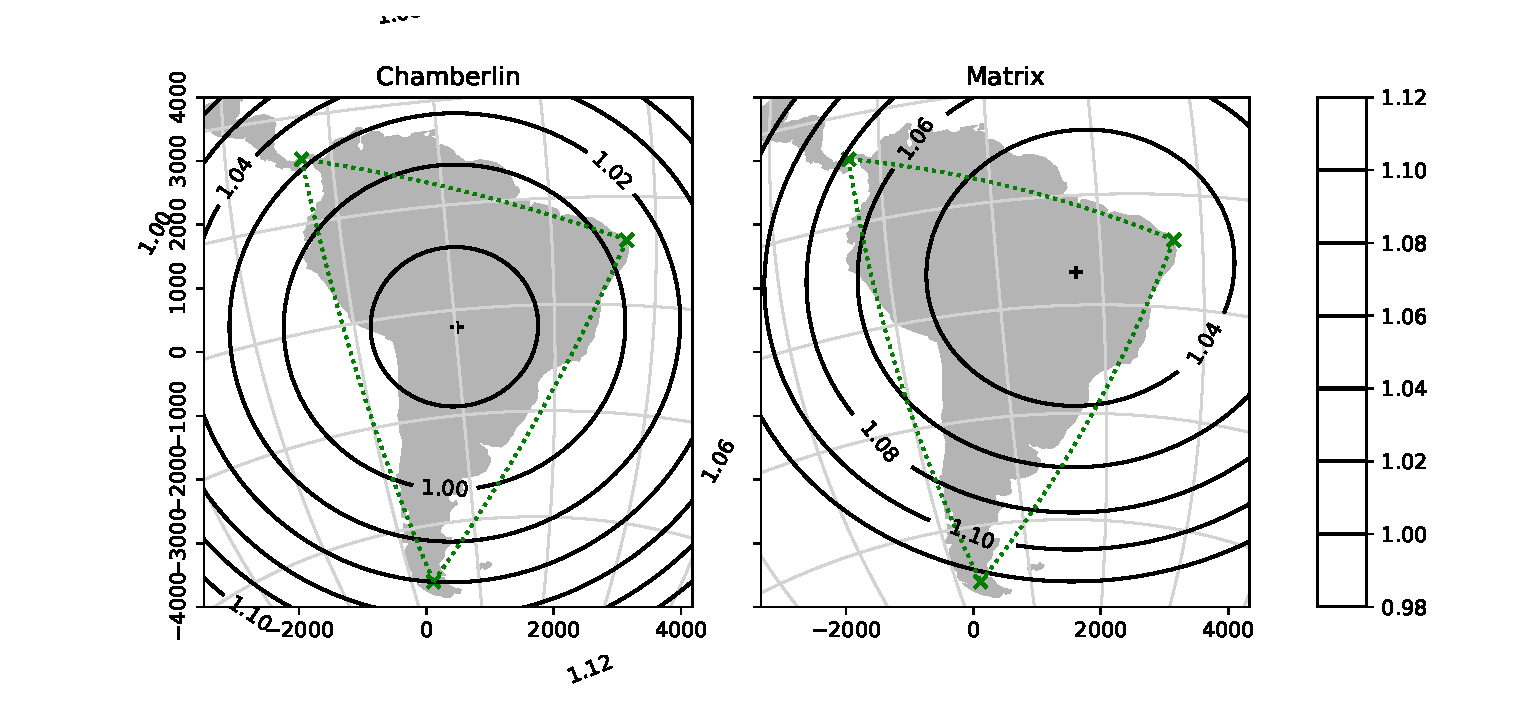
\includegraphics[width=\textwidth]{SA_Wall_Map_scale}
  \caption{Areal scale factor $s$.}
  \label{fig:scale}
\end{figure}

Contour lines of $s$ are shown in Figure \ref{fig:scale}. The contour lines
have the same circular structure in both projections, centered around a
point where $s$ reaches a local minimum. This point is different for each
projection, which influences the differences in aggregate area distortion in
Figure \ref{fig:scalep}.

\begin{figure}%[!htbp]
  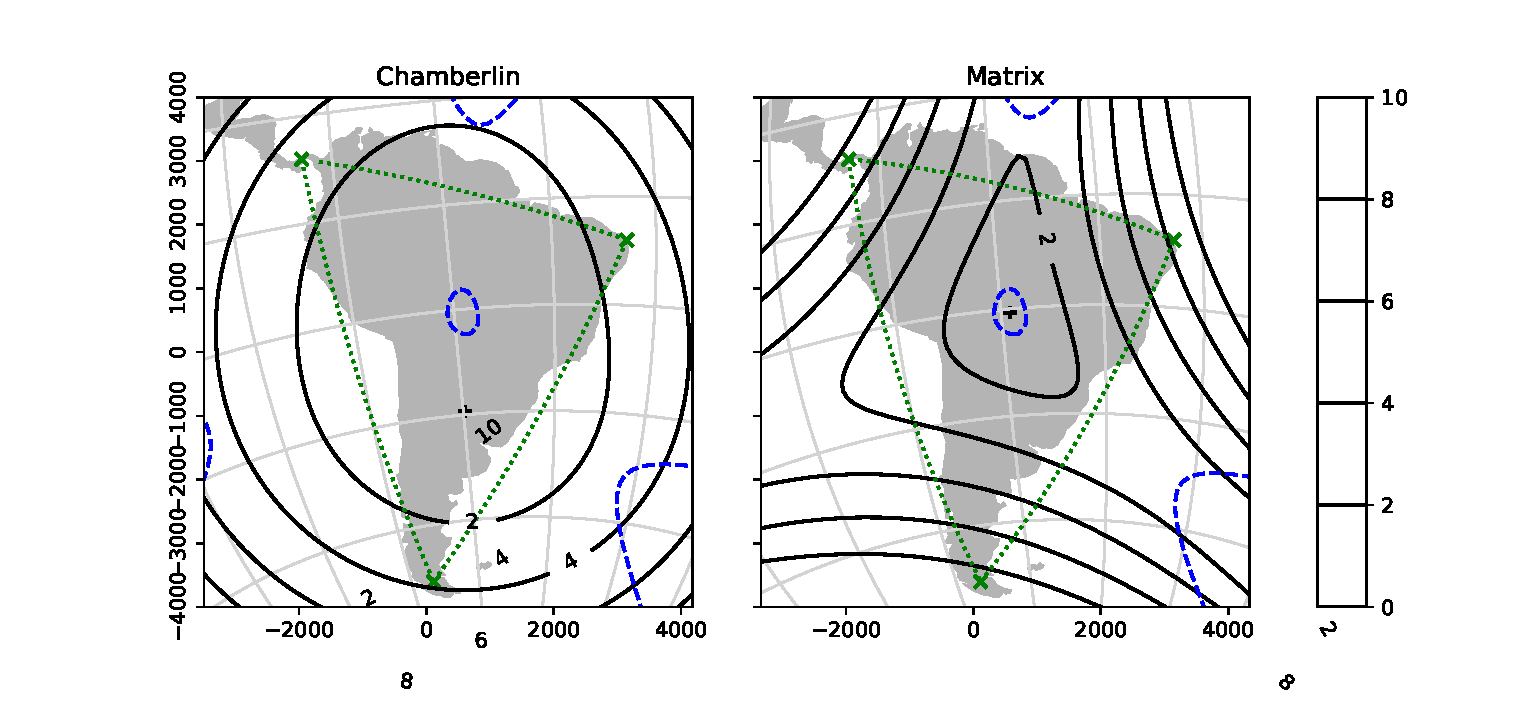
\includegraphics[width=\textwidth]{SA_Wall_Map_omega}
  \caption{Maximum angular deformation $\omega$, in degrees.}
  \label{fig:angle}
\end{figure}

Contour lines of $\omega$ are shown in Figure \ref{fig:angle}. Those in the
Chamberlin projection have an oval shape, while those for the Matrix Trimetric
projection extend outward through each edge of the control triangle.
Both reach a minimum $\omega$ of 0 at a point inside the control triangle.
Highly obtuse control triangles, like Canada Atlas,
may have two local minima for $\omega$ within the control triangle.

\begin{figure}%[!htbp]
  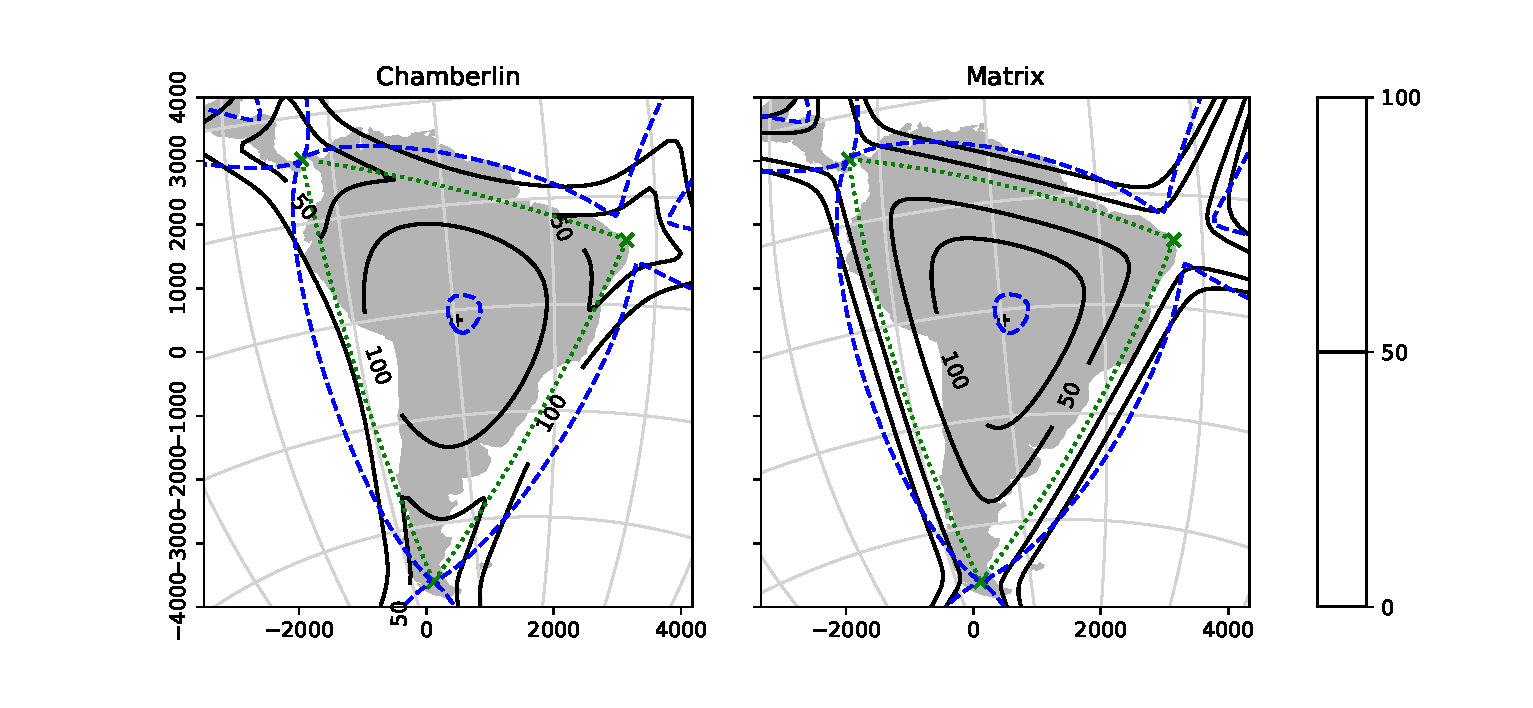
\includegraphics[width=\textwidth]{SA_Wall_Map_distance}
  \caption{Distance deviation $D$.}
  \label{fig:distance}
\end{figure}

Figure \ref{fig:distance} depicts contour lines of $D$ for these two
projections. Both projections have a local minimum of 0 at the control points,
which follows from the geometric construction. Both have a local maximum near
the triangle center. $D$ for the Matrix projection is low along the control
triangle edges, while for the Chamberlin projection it is larger.

In most practical applications the area pictured in these figures will be
sufficient, but it is informative to examine the trend as both projections
extend outward from the control triangle. $s$ increases to a maximum and then
decreases to 0 at the projection boundary. $\omega$ increases to 180 degrees at
the projection boundary, representing the inversion of the overlap region. $D$
increases in general, but for the Matrix Trimetric projection
$D$ remains low on the great circles containing the control triangle edges.

% \subsection{Extremal cases}
% With both projections, points within or near the antipodal triangle may be
% projected so that they overlap points near or within the control triangle. Such
% points can be determined by the areal scale factor: points with positive scale
% factor lie in the usual range of the projection, while those with negative scale
% factor will overlap, and those where the scale factor is 0 lie on the boundary.
% The overlap is projected in the reverse orientation.
%
% For the control triangle used in this text, the overlap area is part of the
% Pacific Ocean, as depicted in Figure \ref{fig:antipodal}. For the Chamberlin
% projection, the area is a rounded triangle surrounding the antipodal triangle,
% while for the Matrix Trimetric projection, it is a three-lobed shape
% where two lobes meet at each vertex of the antipodal triangle.
%
% \begin{figure}%[!htbp]
%
% \caption{Antipodal area. Solid line is Matrix, dashed line is Chamberlin. The
% small triangles inside the dashed line are numerical error.}
% \label{fig:antipodal}
% \end{figure}
%
% Figure \ref{fig:globeproj} shows the projection of the whole globe, including
% the overlap.
% In the Chamberlin projection, the boundary of the overlap is roughly elliptical.
% The boundary of the projection presented here instead has the form of a
% rounded triangle. In general the islands contained in this area are too small
% to be visible in projection, but the Hawaiian islands, which are near the
% northernmost vertex, do appear. On the Chamberlin projection, they are highly
% distorted. On the other projection, one can see that they are reversed.
% For large control triangles approaching a hemisphere, the
% boundary approaches a triangle with straight edges (not pictured).

\section{Conclusion}
We have demonstrated a new compromise map projection, the Matrix Trimetric
projection. The forward formula is given in Equations \ref{eq:forward},
\ref{eq:forwardm}, and \ref{eq:forwardt}. Equation \ref{eq:forward} is a simple
product of a matrix and a vector. The vector depends on the point being
transformed. The matrix calculated by the latter two equations depends only on
the control points, so can be calculated once and reused for any point on the
globe. The forward formula does not have the special cases of the Chamberlin
projection, making it more numerically stable as well as more efficient to
calculate. Comparisons of calculation time were not made:
the Matrix projection would likely be somewhat faster, but for both projections
the bulk of calculation time would be spent in the same distance calculations.

The inverse formula is calculated by Equations \ref{eq:inverse},
\ref{eq:inversem}, \ref{eq:inverser}, \ref{eq:inversev}, and a Newton's method
iteration using Equations \ref{eq:inversefh} and \ref{eq:inversefph} with the
lower bound of Equation \ref{eq:inverseh} as an initial condition. The matrices
in Equations \ref{eq:inversem} and \ref{eq:inversev} also depend only on the
control points, as does matrix $\mathbf A$ in Equations \ref{eq:inversefh} and
\ref{eq:inversefph}, and can be reused. The Chamberlin projection, in contrast,
has no known inverse aside from brute force two-variable inversion.

Figures \ref{fig:omegap}, \ref{fig:distancep}, and \ref{fig:scalep} plot
aggregate measures of distortion within each of the listed control triangles.
The Chamberlin projection outperforms the Matrix projection in terms of
angular distortion and (except in one case) scale distortion, but the reverse
is true for distance distortion. For both projections, distortion tends
to be larger for a larger control triangle. Figures
\ref{fig:proj}--\ref{fig:distance} show the projections applied to South
America, demonstrating the shape of distortions across the mapped area.
Differences between the two projections are small. Apart from the merits of
each of these two projections, this shows the value of compromise projections.
Projections that eliminate one form of distortion often introduce a great deal
of another form of distortion: allowing small amounts of distortion across
multiple measures can produce more attractive maps.

The same control points were used for both projections in this work, but the
optimal placement of control points may be somewhat different for the
application of different projections to the same geographic feature.
The angular distortion of the Matrix Trimetric projection is lower
in a region extending through the middle of the control triangle edges,
so one may wish to orient the triangle to take advantage of that.

The Matrix Trimetric projection is closely related to the Chamberlin projection.
Both are related to the azimuthal equidistant projection and the two-point
equidistant projection, which depend on measurements from a single point and
from a pair of points, respectively.\citep{snyder87} This suggests an
``$n$-metric'' family of projections based on distances from some number of
points. The form of the forward formula suggests a possible family of
projections that are simple functions of such distances, such as a polynomial
function. Additionally, there may exist similar projections using measurements
other than distance, such as area.

The Chamberlin projection implicitly depends on the sphere having nonnegative
curvature: otherwise, the circles in the plane would not be guaranteed to
intersect. While the derivation presented for the Matrix projection uses the
same circles, the formulas are valid for any combination of distances. The
Chamberlin projection can be applied to any surface where distances can be
defined. For instance, the human brain has concave areas. Brain cortex mapping
commonly uses conformal projection,
done using iterative algorithms that are often unstable.\cite{angenent}
If the Matrix projection cannot replace conformal projection for this purpose,
it may be able to provide it with better initial conditions.

An implementation of the Matrix Trimetric projection, as well as code used to
produce the calculations and figures in this text,
is available on the author's Github site.\citep{blind}%\citep{brsrmapproj}


% The Chamberlin projection is only applicable to surfaces of nonnegative
% curvature (or comparable non-differentiable surfaces), since the circles in the
% target plane must overlap. The projection presented here gives a result for all
% possible values of $r_i$, regardless of the relationship among them due to the
% underlying surface. It follows that the Matrix Trimetric projection can be
% applied to any surface possessing a metric: hyperbolic surfaces, toruses, and so
% on. This may have applications to mapping some more esoteric objects in space,
% such as asteroids with concavities.

\bibliographystyle{apacite}
\bibliography{../references}

\end{document}
